\chapter{\'Electronique}

\newpage

\section{Générateur de triangles (Mines-Ponts PSI 2022)}

On considère un générateur de triangles ci-dessous :
\begin{center}
	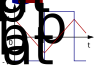
\includegraphics[scale=0.4]{electronique_generateur_triangle.png}
\end{center}
Les trois ALI, nommés respectivement, $(A1)$, $(A2)$ et $(A3)$ sont supposés idéaux. On note $\pm V_{sat}$ la tension de saturation des ALI.

\begin{enumerate}

    \item Après avoir rappelé la définition d'un ALI idéal, indiquer ceux qui fonctionnent en régime linéaire. 

    \item Etablir la relation entre $v_e(t)$ et $v_1(t)$, puis entre $v_1(t)$ et $v_2(t)$.

    \item Déterminer la valeur de $v_s$ selon le sens de variation de $v_2$, puis représenter graphiquement ces variations en reportant $v_s$ en ordonnée et $v_2$ en abscisse. On fera apparaïtre les valeurs remarquables.

    \item Déterminer les variations de $v_2$ et $v_s$ en fonction du temps. Représenter ces variations sur un même graphe. Quelle tension une fonction triangulaire périodique du temps ? Calculer sa période $T$ en fonction de $R$, $C$, $R_1$, $R_2$, $R_3$ et $R_4$.


\end{enumerate}